\chapter{Implementazione}
In questo capitolo viene descritta l'implementazione del nuovo sistema, partendo dai design pattern a cui si è fatto riferimento per lo sviluppo. In seguito, si utilizza la documentazione per definire le API sviluppate e la loro suddivisione in servizi. Si procede con la presentazione dei framework utilizzati per la creazione dei componenti, illustrando le relative parti di codice. Infine si parla della struttura del progetto e dei moduli che lo compongono, analizzando attraverso la simulazione di una chiamata come questi comunicano tra loro.
\label{chap:implementation}

\section{Design Pattern}
\subsection{Inversion of Control}
L'\emph{Inversion of Control (IoC)} è il design pattern su cui si basano la maggior parte dei framework moderni, pertanto il nuovo sistema non rappresenta un'eccezione. Normalmente utilizzando una libreria è il nostro codice a richiamare gli elementi definiti all'interno di essa. Con l'introduzione di questo principio è il nostro codice ad essere richiamato dai componenti del framework, da qui il concetto di \emph{`inversione del controllo'}.

\subsubsection{Façade Pattern}
Questo design pattern contribuisce alla semplificazione delle interazioni con il framework o un set complesso di classi. Quando il codice lavora con un vasto set di oggetti appartenenti a librerie o framework sofisticati, normalmente è necessario inizializzare tali oggetti, tenere traccia delle loro dipendenze e chiamare i relativi metodi nel giusto ordine. In questo modo però il nostro sistema risulta strettamente legato all’implementazione di tali framework rendendolo difficile da mantenere. Il pattern risponde a questo problema. Una Facade è una classe che gestisce al posto nostro la logica appena descritta.

\paragraph{}Si utilizza lo schema del sito \emph{Refactoring Guru} \cite{refactoring:facadepattern} per semplificare i concetti alla base del suo funzionamento. Prendendo come riferimento la Figura \ref{fig:facadepattern} presentiamo gli elementi che compongono il pattern strutturale:

\begin{figure}[H]
    \centering
    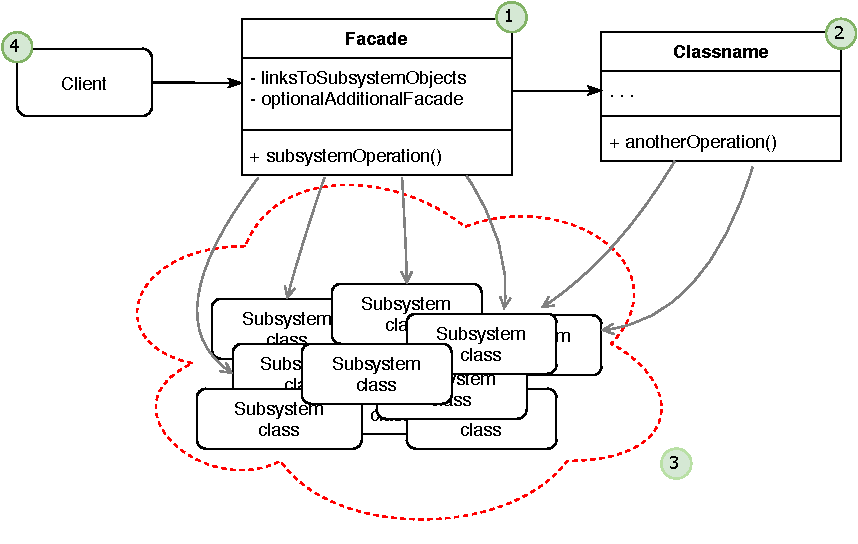
\includegraphics[width=0.65\textwidth]{images/03_1_facade_pattern.pdf}
    \caption{Componenti del Façade Pattern}
    \label{fig:facadepattern}
\end{figure}

\begin{enumerate}
    \item \textbf{Facade}: oggetto che dà accesso al set ristretto di funzionalità del Complex Subsystem
    \item \textbf{Additional Facade}: Facade aggiuntiva nel caso in cui si voglia tenere quella principale il più pulita e semplice possibile
    \item \textbf{Complex Subsytem}: libreria o framework complesso che vogliamo semplificare
    \item \textbf{Client}: Il client fa uso del Complex Subsystem attraverso la Facade
\end{enumerate}

%%%%%%%%%%%%%%%%%%%%%%%%%%%%%%%%%%%%%%%%%%%%%%%%%%%%%%%%%%%%%%%%%%%%%%%%%
\section{Documentazione}
La documentazione è stato il vero primo passo nel percorso di implementazione. Una decisione inusuale per lo sviluppo di un software, ma comprensibile per un caso di refactoring come questo, privo di una documentazione iniziale. 

\subsection{Swagger}
Swagger è un \emph{tool} composto da un set di software open source per progettare, creare e documentare \emph{RESTful APIs} attraverso l’\emph{OpenAPI Specification}, un formato di descrizione apposito per le REST APIs. In particolare aiuta a descrivere:
\begin{enumerate}
    \item \emph{endpoint} presenti e \emph{operazioni CRUD} che è possibile fare su di essi
    \item \emph{parametri} di input e output per ciascuna operazione
    \item metodi di \emph{autenticazione}
    \item informazioni relative al software, come contatti, licenza e termini di utilizzo
\end{enumerate}
Per descrivere il funzionamento del software si è utilizzato \emph{Swagger UI}, un tool che grazie all'uso delle \emph{annotazioni nel codice} e all'integrazione con il framework Spring, permette di creare una pagina web dinamica che presenta tutte le informazioni relative alle API. Ciò che viene mostrato sulla pagina durante l'esecuzione corrisponde alla specifica delle API. Questo documento può essere anche scritto in YAML o JSON: il formato è facile da imparare e comprensibile sia dall'uomo che dalla macchina. 

\begin{figure}[H]
    \centering
    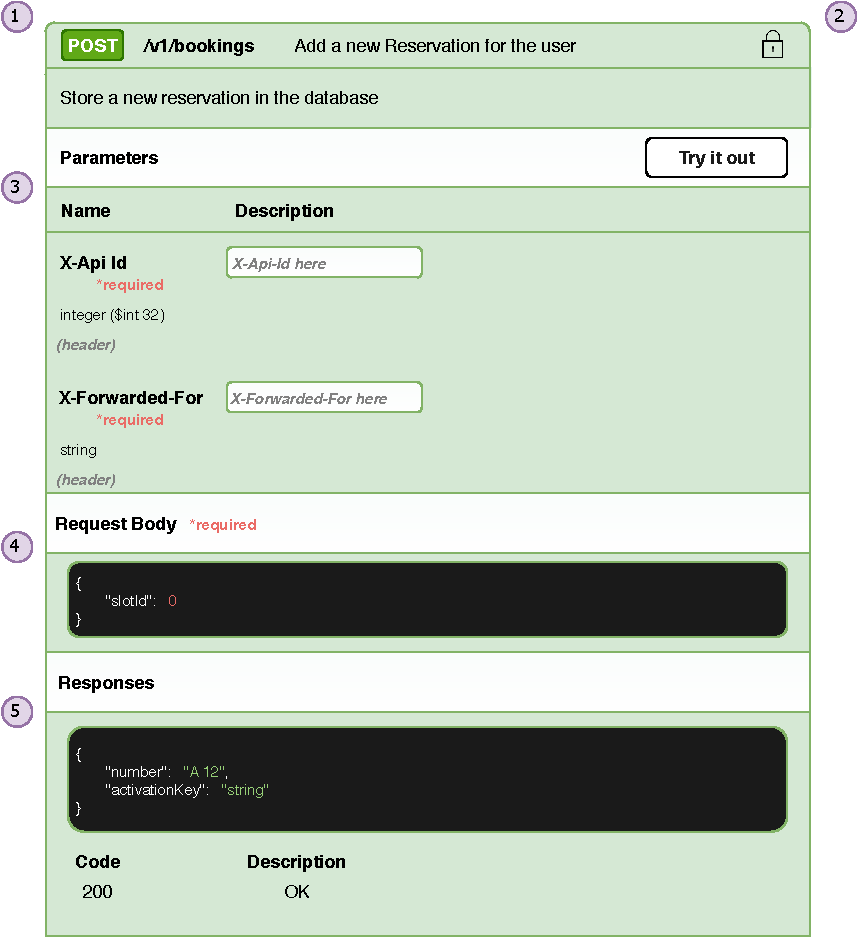
\includegraphics[width=0.87\textwidth]{images/03_2_swaggerui.pdf}
    \caption{Esempio di Specifica OpenAPI}
    \label{fig:swaggerexample}
\end{figure}

In Figura \ref{fig:swaggerexample} viene presentato un esempio di specifica OpenAPI realizzata con Swagger. Il documento descrive l'API di prenotazione di un servizio. In riferimento alla numerazione in figura, elenchiamo i campi che compongono la descrizione della nuova API.
\begin{enumerate}
    \item Metodo HTTP eseguito sull'url \emph{/v1/bookings} dove  \emph{`v1'} indica la versione delle attuali API. In questo campo e nel successivo è presente una breve descrizione dell'operazione.
    \item Il lucchetto in alto a destra, quando presente, indica che per quella chiamata è richiesta un'autorizzazione. In questo caso l'utente per poter prenotare un servizio deve aver effettuato l'accesso al sistema.
    \item In questo campo vengono descritti i parametri e gli header della chiamata. Per ogni parametro viene descritto il suo tipo, e viene aggiunta un informazione che avvisa nel caso questo sia obbligatorio. Di default in tutte le chiamate sono necessari due header: \emph{X-Api-Id} e \emph{X-Forwarded-For}. Il primo passa gli Id API della struttura, così che il sistema sappia sempre quali dati deve mostrare all'utente, mentre il secondo identifica il client che effettua la chiamata al server.
    \item Questa sezione descrive il body del messaggio, se presente. In questo caso la chiamata API viene fatta utilizzando il metodo POST, pertanto è previsto un oggetto JSON nel body della richiesta. L'utente per effettuare una prenotazione invia un oggetto contenente l'ID dello slot che vuole prenotare.
    \item Nel campo viene rappresentato l'oggetto JSON restituito nel caso la richiesta vada a buon fine. È possibile specificare anche altri codici di risposte che è possibile ricevere.
\end{enumerate}

\subsection{Nuove API}
Sono state individuate un totale di 6 API associabili al \emph{booking server}, tutte originariamente sviluppate come metodi \emph{GET}. Parte di queste API, oltre alle operazioni sul database, comprendono un sistema di notifica utente. Per queste API si è deciso di separare le due operazioni, delegando il sistema di notifica al \emph{Communication Server}.
\begin{figure}[H]
    \centering
    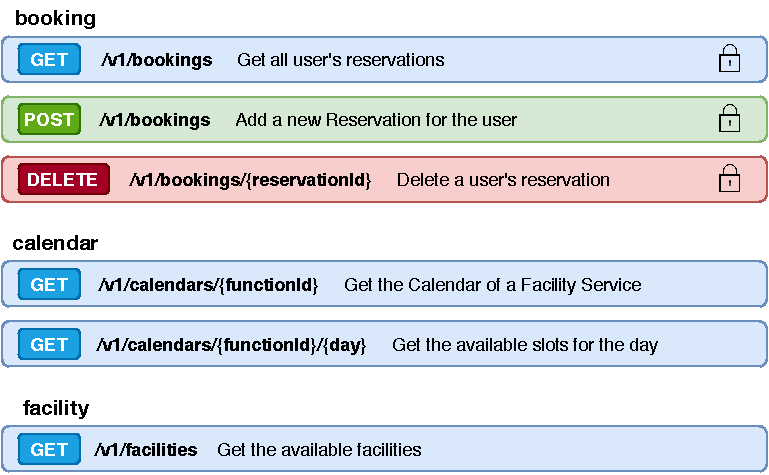
\includegraphics[width=0.99\textwidth]{images/03_3_new_rest_api.pdf}
    \caption{Nuove API REST}
    \label{fig:newrestapi}
\end{figure}

In riferimento alla Figura \ref{fig:newrestapi}, vengono ora elencate le operazioni svolte dalle nuove API REST in ordine di servizio: \emph{booking service}, \emph{calendar service}, \emph{facility service}.
\begin{itemize}
    \item \texttt{GET v1/bookings} recupera le prenotazioni di un utente. Questa operazione richiede un utente autenticato al sistema. Viene chiamata quando l'utente effettua il login o il numero delle sue prenotazioni cambia, come ad esempio dopo una prenotazione andata a buon fine o dopo una sua cancellazione.
    \item \texttt{POST v1/bookings} registra una nuova prenotazione nel database. Questa richiesta è inviata al booking server nel momento in cui l'utente prenota un servizio. Si tratta di una richiesta fatta con il metodo POST, pertanto è previsto l'invio di un oggetto nel \emph{body della richiesta}. Nell'\emph{oggetto Reservation} mandato nella richiesta viene specificato lo \emph{slot} che l'utente vuole prenotare.
    \item \texttt{DELETE v1/bookings/\{reservationId\}} il metodo delete viene utilizzato nel momento in cui un utente sceglie di eliminare una prenotazione. Nella richiesta viene specificata una \emph{variabile di percorso}, la quale sta a indicare l'ID della prenotazione che l'utente vuole cancellare.
    \item \texttt{GET v1/calendars/\{functionId\}} restituisce alla pagina i dati relativi al calendario di prenotazione di un servizio (chiamato per l'appunto \emph{function di una facility}). Il parametro in questo caso rappresenta l'ID del servizio di una struttura. Il calendario viene restituito in termini di data: giorno, mese, anno.
    \item \texttt{GET v1/calendars/\{functionId\}/\{day\}} restituisce gli slot disponibili per un determinato giorno appartente al calendario. Può essere considerato come un'estensione del percorso precedente. Ciascuno slot corrisponde a una \emph{fascia oraria} che l'utente può prenotare. L'ID dello slot verrà poi incapsulato dentro un oggetto nel momento in cui l'utente procede con la sua prenotazione, e inserito nel body della relativa richiesta in POST. Gli slot vengono mostrati in termini di orario: ora e minuti. 
\end{itemize}

%%%%%%%%%%%%%%%%%%%%%%%%%%%%%%%%%%%%%%%%%%%%%%%%%%%%%%%%%%%%%%%%%%%%%%%%%
\section{Spring Framework}
\epigraph{«Un framework open source nato con l’intento di gestire la complessità nello sviluppo di applicazioni enterprise.»}{Team di Sviluppo di Spring}

Spring è un framework “leggero” e grazie alla sua architettura estremamente modulare é possibile utilizzarlo nella sua interezza o solo in parte, in quanto non sconvolge l'architettura esistente. Il framework mette a disposizione \emph{una serie completa di strumenti} atti a gestire l’intera complessità di un progetto software. In particolare, fornisce un approccio semplificato alla maggior parte dei problemi ricorrenti nello sviluppo software: accesso al database, gestione delle dipendenze e testing.

\subsection{Dependency Injection}
La \emph{Dependency Injection (DI)} è una delle diverse implementazioni che la \emph{Inversion of Control} può avere. Spring implementa la \emph{IoC} tramite Dependency Injection. La \emph{DI} prevede che tutti gli oggetti all’interno della nostra applicazione accettino le dipendenze, ovvero gli oggetti di cui hanno bisogno, tramite costruttore o metodi setter. Non sono quindi gli stessi oggetti a creare le proprie dipendenze, ma queste vengono `iniettate' dall’esterno.

\subsection{Annotazioni}
La dichiarazione dei componenti (da ora chiamati \emph{bean}), come in generale la configurazione di un’applicazione Spring, può avvenire in tre modi differenti: tramite \textit{file XML}, \textit{classi di configurazione}, oppure \textit{annotazioni Java}. Di seguito si fa riferimento alle principali annotazioni utilizzate durante l'implementazione nel codice Java:
\begin{itemize} 
    \item \texttt{@Controller} gestisce le interazioni tra utenti e logica di business. Riceve comandi ed espone le informazioni in modo che siano comprensibili per l’utente o utilizzabili da altri sistemi. Nel codice è stata utilizzata l'annotazione \emph{@RestController} (un alias di questa annotazione) per fare riferimento alle classi di controllo dei servizi \textit{BookingController, CalendarController e FacilityController}.
    \item \texttt{@Service} gestisce la logica di business. Ha la funzione di elaborare i dati e di fornirli ai Controller per essere esposti verso il client. Allo stesso tempo, le informazioni da salvare vengono inviate allo strato di accesso ai dati. Questa annotazione è stata utilizzata nelle classi \textit{BookingService, CalendarService e FacilityService}, dove venivano implementati i metodi chiamati dalle REST API.
    \item \texttt{@Autowired} può essere applicata a diversi elementi della classe: un campo, un metodo o un costruttore. Lo scopo dell'annotazione è quello di indicare a Spring quali sono le dipendenze richieste da un determinato oggetto. Queste vengono ricercate tra le istanze presenti nell'IoC container e, se presenti, vengono `iniettate' mediante il costruttore o il metodo annotato. Un esempio di implementazione di questa annotazione la si ha nelle classi \emph{Service}, dove per comunicare con il database nel costruttore si istanzia la relativa classe \textit{Data Access Object}, che invece presenta l'annotazione \emph{Service}.
\end{itemize}

%%%%%%%%%%%%%%%%%%%%%%%%%%%%%%%%%%%%%%%%%%%%%%%%%%%%%%%%%%%%%%%%%%%%%%%%%
\section{MyBatis}
MyBatis è un framework di persistenza che effettua il mapping (ovvero definisce la corrispondenza) tra i metodi Java e le query SQL. Per farlo, mappa le tabelle presenti sul proprio database con delle classi Java, servendosi di un file di configurazione in linguaggio XML. Le query SQL ovviamente rimangono comunque a carico del programmatore. Il framework si limita a semplificare l’interfacciarsi del codice con il database. Le query vengono inserite in un \emph{file di mapping in formato XML}, nel quale oltre al \textit{comando da eseguire} è necessario specificare le associazioni, ovvero le tabelle che interessano l'operazione sul database.

\subsection{Configurazione}
\usemintedstyle{autumn}
\begin{figure}[H]
    \inputminted[firstline=6, lastline=35]{octave}{src/MyBatis/MyBatisGenerator.xml}
    \caption{File di Configurazione di MyBatis}
    \label{fig:mybatisconfiguration}
\end{figure}

In Figura \ref{fig:mybatisconfiguration} viene mostrato il file XML contenente la configurazione di MyBatis. Nel file individuiamo diversi tag:
\begin{itemize}
    \item <jdbcConnection> comprende le informazioni di connessione al database. Nel codice mostrato le informazioni sensibili sono state anonimizzate.
    \item \texttt{<table>} specifica una tabella di cui mi MyBatis andrà a effettuare il mapping.
    \item \texttt{<sqlMapGenerator>} specifica il percorso in cui vengono salvati i file XML che mappano una specifica tabella e le sue query.
    \item \texttt{<javaClientGenerator>} specifica il percorso in cui vengono salvate le interfacce corrispondenti ai file XML.
\end{itemize}

Una volta creato il file di configurazione questo viene passato come input al tool di MyBatis, che procede a effettuarne il mapping appena configurato.

\subsection{Creazione di una Query}
\usemintedstyle{autumn}
\begin{figure}[H]
    \inputminted[firstline=3, lastline=30]{octave}{src/MyBatis/ServicesExMapper.xml}
    \caption{Query con MyBatis}
    \label{fig:mybatisquery}
\end{figure}
In Figura \ref{fig:mybatisquery} viene rappresentata la sruttura del file \emph{ConfigServicesRemoteExMapper.xml}, che eredita dalla classe padre \emph{ConfigServicesRemoteMapper.xml}. Per i file XML contenti le query delle API si è scelto di utilizzare il suffisso `ex', in modo da non modificare i file generati da MyBatis, ma limitandosi ad \emph{estendere le loro funzionalità}. La query in figura rappresenta una semplice \emph{JOIN} tra \emph{struttura} e \emph{servizio erogato}. Nel file vengono specificate eventuali associazioni presenti nella query tra la tabella padre e altre tabelle (in questo caso \textit{ConfigMryouEnterprise}, dove sono salvate le strutture). Nel tag \texttt{<select>} vengono specificati \emph{l'attributo id}, che mappa la query, e l'attributo \emph{parameterType}. Quest'ultimo attributo serve per specificare la classe che istanzia l'oggetto che gestisce i parametri inseriti nelle clausole \textit{Group By, Order By, Where}.


\begin{figure}[H]
\usemintedstyle{colorful}
    \begin{minted}{JAVA}
    @Mapper

    public interface ConfigServicesRemoteExMapper 
        ConfigServicesRemote selectByFilter(ConfigServicesRemoteFilter filter);
    }    
    \end{minted}
    \caption{Interfaccia ConfigServicesRemoteExMapper}
    \label{fig:mybatismapperinterface}
\end{figure}
Una volta creato il file XML, è necessario creare il mapper Java. Il Mapper, come si osserva in Figura \ref{fig:mybatismapperinterface}, è un'interfaccia contenente i metodi corrispondenti agli ID delle query create. Il metodo in questo caso restituisce un unico oggetto \textit{ConfigServicesRemote}. È possibile fare restituire alle query anche una lista o oggetti come date, stringhe o interi. Il tipo di oggetto risultante deve sempre essere specificato nel mapper XML. In questo caso, per interrogare il sistema, il database ha bisogno di un oggetto ConfigServicesRemoteFilter, creato ad-hoc per semplificare la costruzione della query. La classe di quest'oggetto è costituita da attributi con metodi setter per specificarne il valore. In questo modo, cercando un servizio con uno specifico ID, sarà sufficiente scrivere quanto segue in Figura \ref{fig:filterobject}:

\begin{figure}
    \begin{minted}{JAVA}
        ConfigServicesRemoteFilter serviceFilter; 
        serviceFilter = new ConfigServicesRemoteFilter();
        serviceFilter.setAndConfigServicesRemoteIdEqualsTo(50);
    \end{minted}
    \caption{ConfigServicesRemoteFilter Object}
    \label{fig:filterobject}
\end{figure}

L'oggetto creato è ora pronto per essere passato al metodo \texttt{selectByFilter}. Così facendo, la query creata nel Mapper XML interroga il database specificando un service ID con valore pari a 50. Le query sono state tutte costruite seguendo questa logica. Nonostante il processo possa sembrare macchinoso sotto certi aspetti, l'utilizzo di MyBatis ha semplificato di molto la comunicazione con il database.

%%%%%%%%%%%%%%%%%%%%%%%%%%%%%%%%%%%%%%%%%%%%%%%%%%%%%%%%%%%%%%%%%%%%%%%%%
\section{Struttura del Progetto}
In questa sezione viene presentato il packaging del progetto. Si presentano i moduli che lo compongono e le loro interazioni, simulando l'operazione di chiamata di una REST API. All'interno del progetto distinguiamo 3 moduli principali, ciascuno con funzionalità diverse:
\begin{itemize}
    \item \textbf{booking-dto}: contiene le classi utilizzate per istanziare gli oggetti utilizzati nei body delle richieste POST del client, o per istanziare gli oggetti restituiti dal server.
    \item \textbf{booking-persistance}: comprende le classi di persistenza, ovvero tutte quelle classi di Mapping e configurazione delle tabelle del database, nonchè i file XML necessari al corretto funzionamento di MyBatis.
    \item \textbf{booking-server}: contiene le vere e proprie API REST. In questo modulo sono contenute le classi Controller delle API, con i relativi servizi dove vengono implementate le chiamate. In riferimento alla Figura \ref{fig:newrestapi} individuiamo 3 controller, ai quali corrispondono i 3 servizi: \emph{booking}, \emph{calendar} e \emph{facility}.
\end{itemize}

\subsection{Data Transfer Object - DTO}
Il \emph{Data Transfer Object} è un design pattern utilizzato per trasferire dati tra sottosistemi di un'applicazione software. Nel processo di implementazione, il DTO è stato utilizzato per mappare gli oggetti restituiti dalle query del DAO, in oggetti con cui l'utente può interagire. In questo modo il risultato di una query che sul database interessa diverse tabelle viene presentato all'utente come un singolo oggetto che può comprendere.

\subsubsection{Class Diagram}
In Figura \ref{fig:classdiagram} viene presentato il diagramma delle classi utilizzate per il mapping dei risultati ottenuti dalle query. Nelle sezioni successive si farà riferimento a questi oggetti. I diversi colori utilizzati rappresentano la suddivisione in servizi. Le classi che non sono state colorate istanziano oggetti che non sono direttamente utilizzati nelle richieste o restituiti nelle risposte dalle chiamate REST.
\begin{figure}[H]
    \centering
    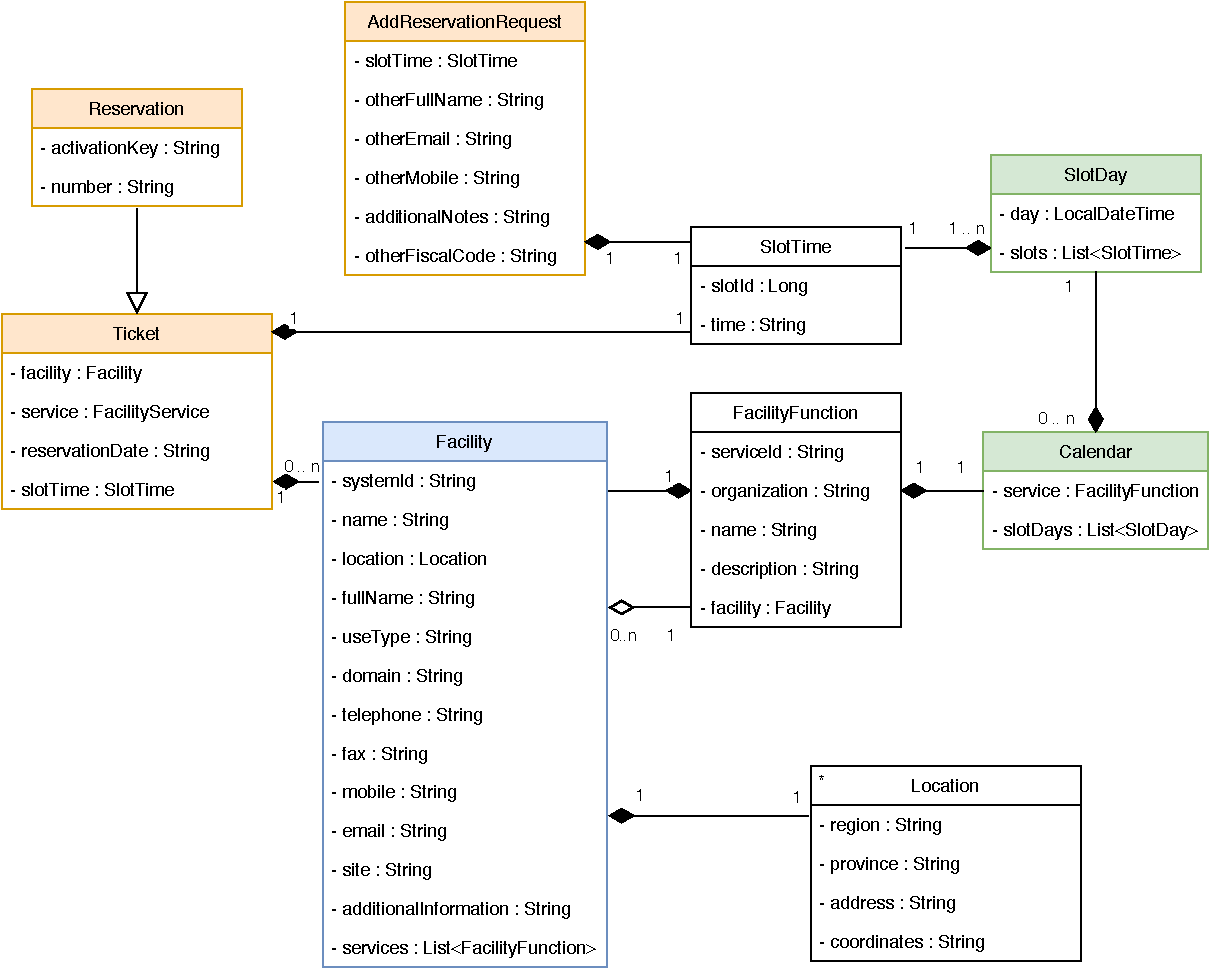
\includegraphics[width=0.98\textwidth]{images/03_4_class_diagram.pdf}
    \caption{DTO Class Diagram}
    \label{fig:classdiagram}
\end{figure}

\subsection{Data Access Object - DAO}
Il \emph{Data Access Object} rappresenta un pattern architetturale per la gestione della persistenza. Seguendo questo design pattern, è possibile trovare nell'omonimo modulo un set di classi atte a disaccoppiare il server dall'accesso al database. Il DAO gestisce l'interazione tra i servizi REST e l'accesso al database mediato dai mapping realizzati con MyBatis, nascondendone i passaggi implementativi.

\begin{figure}
\begin{minted}{Java}
@Service
public class ConfigMryouEnterpriseDao {    
private ConfigMryouEnterpriseExMapper mapper;

@Autowired
public ConfigMryouEnterpriseDao(ConfigMryouEnterpriseExMapper mapper) {
    this.mapper = mapper;
}

public List<ConfigMryouEnterpriseEx> findAll() {
    ConfigMryouEnterpriseExample example = new ConfigMryouEnterpriseExample();
    return mapper.selectExByExample(example);    
}

public List<ConfigMryouEnterpriseEx> findActive      
                        (ConfigMryouEnterpriseFilter filter) {
    return mapper.selectByFilter(filter);
}
\end{minted}
\caption{Classe ConfigMryouEnterpriseDao}
\label{fig:daoclass}
\end{figure}

La classe ConfigMryouEnterpriseDao in Figura \ref{fig:daoclass} viene utilizzata per interfacciarsi con il file di mapping XML creato seguendo la procedura precedentemente esposta. La query chiamata restituisce la lista delle strutture sanitarie, sulla base dell'ID API fornito. L'ID API è un \emph{parametro della query}, che può essere assegnato mediante il relativo metodo setter della classe \emph{ConfigMryouEnterpriseFilter}. La classe utilizza le annotazioni Spring per comunicare con gli altri componenti dell'applicazione.

\subsection{Booking Server}
All'interno di questo modulo sono presenti le \emph{classi controller} e le relative \emph{classi service}. Le prime contribuiscono a creare la documentazione Swagger, e quindi le specifiche Open Api (Figura \ref{fig:swaggerexample}), mentre le seconde implementano la chiamata REST.

\subsubsection{Classi Controller}
La classe \emph{FacilityController} (Figura \ref{fig:facilitycontroller}) presenta la chiamata \texttt{GET v1/facilities}: il metodo HTTP che restituisce la lista delle strutture sanitarie. La chiamata è implementata richiamando il metodo dell'omonima \emph{classe service} all'interno della funzione exec.
\begin{figure}
\begin{minted}{Java}
    @RestController
    @RequestMapping(value = "/v1/facilities",
                    produces = {MediaType.APPLICATION_JSON_VALUE})

    public class FacilityController {
        private final FacilityService facilityService;
    
        @Autowired
        public FacilityController(FacilityService facilityService) {
            this.facilityService = facilityService;
        }
    
        @SecurityRequirements
        @GetMapping
        @Operation(summary = "Get all available facilities", 
                description = "Returns all the available facilities",
                tags = {"facility"})
        @ApiResponses(value = {
                @ApiResponse(responseCode = "404", 
                             description = "Facilities not found"),})
        public Result<Facility> facilities(@RequestHeader("X-Api-Id")    
                                                Integer apiId,
                                           @RequestHeader ("X-Forwarded-For") 
                                                String forwardedFor,
                                           @RequestParam(name = "lang", 
                                            required = false, 
                                            defaultValue = "")  String lang) {
            return exec("get-facilities", 
                () -> facilityService.find(apiId, forwardedFor, lang));
        }
    }
\end{minted}
\caption{Classe FacilityController}
\label{fig:facilitycontroller}
\end{figure}

\subsubsection{Classi Service}
A questo punto si conoscono i vari componenti del sistema. I principali componenti che gestiscono la \emph{logica dietro a una chiamata REST} vengono dichiarati come \emph{dipendenze nel costruttore} della classe service. In seguito, queste istanze chiamano le loro funzioni all'interno del metodo che implementa la chiamata. Il service non si limita a preparare l'oggetto della risposta. In questa classe sono analizzati i parametri della richiesta (headers inclusi), e sono lanciate eccezioni se durante l'esecuzione si verifica un problema. Analizziamo il codice della classe \emph{FacilityService}, che comunica con i componenti appena esposti.

In Figura \ref{fig:facilityservice} viene mostrata l'implementazione della chiamata \texttt{GET v1/facilities}. Com'è logico pensare la classe utilizza le annotazioni Spring per legarsi alla classe ConfigMryouEnterpriseDao (illustrata precedentemente) e al DtoMapper, una classe creata appositamente per convertire gli oggetti mappati sui file XML di MyBatis in oggetti definiti nel DTO (Figura \ref{fig:classdiagram}). Nella classe viene prima creato il filtro come visto in Figura \ref{fig:filterobject} e successivamente chiamata la query definita nel classe DAO (Figura \ref{fig:daoclass}). Se il risultato della query ha una struttura particolarmente difficile per essere convertito dal DTO, può essere passato al DaoHelper come in questo caso. Il DaoHelper è una classe che ha il compito di separare gli oggetti risultanti dalle query con una o più condizioni di join. Così facendo è possibile fornire al DtoMapper anche due oggetti distinti, facilitandone la conversione. Il nuovo oggetto restituito dal DtoMapper viene in seguito incapsulato in una \emph{lista Result}, che contiene due elementi: la lista contenente gli oggetti restituiti dal mapper (in questo caso sono oggetti Facility) e il numero totale degli elementi della lista.
\begin{figure}
\begin{minted}{Java}
@Service
public class FacilityService {
    private static final Logger LOG = getLogger(FacilityService.class);
    private final ConfigMryouEnterpriseDao configMryouEnterpriseDao;
    private final DtoMapper dtoMapper;

    @Autowired
    public FacilityService(ConfigMryouEnterpriseDao configMryouEnterpriseDao,
                           DtoMapper dtoMapper) {
        this.configMryouEnterpriseDao = configMryouEnterpriseDao;
        this.dtoMapper = dtoMapper;
    }

    public Result<Facility> find(Integer apiId, String forwardedFor, 
                                                String lang) {
        LOG.debug("Looking for facilities [apiId={}, forwardedFor={}]", 
                                            apiId, forwardedFor);
        ConfigMryouEnterpriseFilter filter = new ConfigMryouEnterpriseFilter();

        // filter settings
        filter.setAndIsActive(true);
        filter.setAndApiKey(apiId);
        filter.setAndVisibleInWeeks(1);
        filter.setGroupByClause("CME.id, CSR.id");
        filter.setOrderByClause("CME.id, CSR.id");

        List<ConfigMryouEnterpriseEx> enterprises;
        enterprises = configMryouEnterpriseDao.findActive(filter);

        List<Tuple2<ConfigMryouEnterprise, List<ConfigServicesRemote>>> 
                            orderedEnterprises =
                DaoHelper.orderFacilities(enterprises);

        List<Facility> ret = orderedEnterprises.stream()
                .map(t -> dtoMapper.copy(t.first(), t.second(), lang))
                .collect(Collectors.toList());
        return new Result<>(ret, ret.size());

    }
}
\end{minted}
\caption{Classe FacilityService}
\label{fig:facilityservice}
\end{figure}
%%%%%%%%%%%%%%%%%%%%%%%%%%%%%%%%%%%%%%%%%%%%%%%%%%%%%%%%%%%%%%%%%%%%%%%%%

%%%%%%%%%%%%%%%%%%%%%%%%%%%%%%%%%%%%%%%%%%%%%%%%%%%%%%%%%%%%%%%%%%%%%%%%%